\documentclass[letterpaper]{article} % DO NOT CHANGE THIS
\usepackage[submission]{aaai2027}  % DO NOT CHANGE THIS
\usepackage[hyphens]{url}  % DO NOT CHANGE THIS
\usepackage{graphicx} % DO NOT CHANGE THIS
\usepackage{natbib}  % DO NOT CHANGE THIS
\usepackage{caption} % DO NOT CHANGE THIS
\usepackage{amsmath}
\usepackage{amssymb}
\usepackage{booktabs}
\frenchspacing  % DO NOT CHANGE THIS
\setlength{\pdfpagewidth}{8.5in} % DO NOT CHANGE THIS
\setlength{\pdfpageheight}{11in} % DO NOT CHANGE THIS

\newcommand{\method}[1]{\texttt{#1}}

% AAAI-27 compressed version of the Q/R/M/C measurement-framework
% manuscript.  The full single-column version (42 pp.) is the
% Supplementary Document; this file keeps 7 pages of technical content
% per the compression plan (docs/AAAI_COMPRESSION_PLAN.md, revised
% 2026-07-04: the external-framework validation moved INTO the body).

\pdfinfo{
/TemplateVersion (2027.1)
}

\title{Q/R/M/C: A Stage-Decomposition Evaluation Protocol\\for Memory-Based Agents}
\author{Anonymous submission}
\affiliations{Anonymous submission}

\begin{document}

\maketitle

\begin{abstract}
Success-only metrics collapse qualitatively different memory failures
into a single scalar, hiding \emph{which stage} of the retrieval
pipeline is responsible. We contribute an evaluation protocol: the
Q/R/M/C decomposition (Query formation, Retrieval satisfaction, target
Materialization, Completion), operationalised so that four conditional
rates are computable from standard trajectory logs. The arithmetic is
the chain rule, deliberately so --- like precision/recall, the value is
identifiability and what the decomposition reveals. Single-agent
(MiniGrid, BabyAI): oracle-stage interventions localise a
retrieval-limited task ($0.39\!\to\!0.60$ under oracle retrieval) vs.\
downstream-limited ones, and log inspection refines the diagnosis ---
candidate \emph{ranking} is near-optimal ($96.9\%$) while candidate
\emph{generation} fails at $91\%$ of decision points: a
memory-accumulation limit. Multi-agent (35{,}640 runs, four sharing
architectures, cadence $K$): the predicted bottleneck shift between
Materialization and Completion is confirmed as cluster-robust slopes
(Spearman $-0.53$/$+0.43$), time-to-success has an interior optimum at
$K{=}8$, and a provenance annotation supplies the mechanism --- the
completion collapse of fast sharing concentrates in locks backed by
foreign evidence. Externally, the identical tool-trace contract
instruments three third-party agent stacks (OpenAI SDK, LangGraph,
AutoGen): engineered structural failures localise identically on every
stack ($R^\star{=}0$, $C^\star{=}0$ in $20/20$), while on clean tasks
the frameworks spread $0.50$--$0.75$ end-to-end and the stages
attribute the spread to weak first-commitment discipline with
different recovery loops. The protocol makes memory failures
comparable across symbolic, learned, LLM, single- and multi-agent
systems.
\end{abstract}

\section{Introduction}

Embodied, goal-conditioned, and LLM agents increasingly retrieve
places, objects, and facts \emph{by meaning} from an explicit memory,
yet are evaluated almost exclusively end-to-end: if success improves,
memory is judged useful. Two systems with the same success rate can
fail for entirely different reasons --- one never accumulates
queryable evidence, another retrieves perfectly and loses the target
to a peer. This paper contributes the measurement instrument that
separates such cases.

The instrument is a four-stage decomposition of memory-based task
completion: \textbf{Q}uery formation (the planner emits a semantic
intent), \textbf{R}etrieval satisfaction (memory returns a candidate
matching the task), target \textbf{M}aterialization (the planner locks
one candidate as an actionable target), and \textbf{C}ompletion (the
controller reaches it). Logged as per-episode events
$Q^\star,R^\star,M^\star,C^\star$, they factorise semantic-path
completion into conditional rates estimable from ordinary trajectory
logs (Definition~1; a multi-agent extension with memory and occupancy
coupling channels is Definition~2). The consistency argument is the
chain rule plus frequency estimation, and we claim no mathematical
novelty for it: exactly as decomposing accuracy into precision and
recall added no mathematics but changed what the field could see, the
contribution is a \emph{logging discipline} and what it reveals.

\paragraph{Contributions.}
\begin{enumerate}
\item \textbf{The protocol.} Operational, log-level definitions of the
  four stage events for single agents (Definition~1) and communicating
  collectives (Definition~2), with identifiability under a stated
  conditional stage-Markov assumption, plus a stress test of that
  assumption.
\item \textbf{Diagnoses that success cannot make.} Single-agent:
  oracle-stage interventions and log forensics attribute failures to
  memory \emph{accumulation} rather than ranking. Multi-agent: a
  registered slope-level claim (Empirical Claim~1) --- fast sharing
  raises $P(M^\star|R^\star)$ and lowers $P(C^\star|M^\star)$ --- is
  confirmed on a 35{,}640-run sweep, with an interior time-to-success
  optimum at $K{=}8$ and a provenance-level mechanism.
\item \textbf{External validity.} The same contract, defined once over
  tool traces, instruments OpenAI-SDK, LangGraph, and AutoGen agents
  without per-framework adaptation; engineered structural failures
  localise identically on all stacks, and behavioural differences
  between stacks are attributed stage-by-stage.
\end{enumerate}

\begin{table}[t]
\caption{The paper's argument in miniature: one logging contract, five
system classes, a located diagnosis in each. Every section
instantiates one row.}
\label{tab:portability}
\centering
\small
\setlength{\tabcolsep}{3pt}
\begin{tabular}{p{2.5cm} p{5.4cm}}
\toprule
System class & What the same four events revealed \\
\midrule
Symbolic single agent & ranking $96.9\%$ vs.\ empty candidates $91\%$: an \emph{accumulation} limit \\
Symbolic collective & M$\leftrightarrow$C bottleneck shift; $t_{\mathrm{succ}}$ optimum $K{=}8$; provenance mechanism \\
Learned policies & competitive success, collapsed stage observability \\
LLM agents & $1.00\!\to\!0.00$ collapse $=$ pure C-budget; sharing lowers success $2/3\!\to\!1/3$ \\
Third-party stacks $\times$ 2 models & structural failures localize identically; $M_1$ separates models; frameworks reshape it \\
\bottomrule
\end{tabular}
\end{table}

\noindent\fbox{\parbox{0.97\columnwidth}{\small
\textbf{Scope and non-claims.} (i)~No mathematical novelty in the
factorisation; the contribution is operationalisation. (ii)~Empirical
Claim~1 is a verified slope-level observation, not a theorem. (iii)~No
claim about the conditional product $\Phi$ (monotone in our data); the
interior optimum lives on time-to-success. (iv)~Primary substrates are
grid worlds; a continuous-state check (VMAS) is directional; LLM
studies use local models at modest $n$. (v)~Multi-agent place identity
assumes a shared coordinate frame; a companion manuscript removes it.
(vi)~The protocol unifies \emph{observation points}, not
representations --- but $R^\star$ and $M^\star$ presuppose an
entity-correspondence oracle between memory content and world
referents (here supplied by instrumented environments); without it the
protocol degrades gracefully to $Q^\star$ and $C^\star$. Grounding
that correspondence is open.
}}

\section{The Q/R/M/C Protocol}
\label{sec:protocol}

An episode issues a semantic query $q$ (required/preferred/penalty
tags); memory returns candidates; the planner locks one; the
controller executes. The four events anchor at logged triggers:
$Q^\star$ fires on intent emission; $R^\star$ when the candidate set
contains a task-satisfying candidate; $M^\star$ on lock acquisition of
a true target; $C^\star$ on arrival. Per-episode flags are ORs over
ticks; conditional rates $P(R^\star|Q^\star)$, $P(M^\star|R^\star)$,
$P(C^\star|M^\star)$ are frequency estimates over episodes.

\textbf{Definition 1} (single-agent estimability, informal). Under a
conditional stage-Markov property --- each stage outcome depends on
the trace only through its predecessor stage --- semantic-path
completion factorises as
$P(C^\star) = P(Q^\star)\,P(R^\star|Q^\star)\,P(M^\star|R^\star)\,
P(C^\star|M^\star)$, and each factor is consistently estimable from
logs. A simulation stress test quantifies estimator bias when the
assumption is violated by a hidden confounder: $P(M^\star|R^\star)$
stays unbiased while $P(C^\star|M^\star)$ inflates, so diagnoses that
hinge on the M--C \emph{contrast} degrade gracefully (supplement).

\textbf{Definition 2} (multi-agent extension, informal). With $N$
agents sharing memory by peer broadcast every $K$ ticks, the
conditioning sets enlarge with two coupling channels: the shared
memory $\mathcal{M}^{(K)}_{-i}$ and occupancy $\mathcal{O}_{-i}$
(scarce targets are consumed). The same four rates are logged per
agent.

\textbf{Empirical Claim 1} (bottleneck shift, slope-level). As $K$
decreases (faster sharing), $P(M^\star|R^\star)$ rises --- fresher
peer evidence enables reliable commitment --- and $P(C^\star|M^\star)$
falls --- peers race for the same targets. Both are claims about
conditional rates, not about their product.

Interpretive readings of the stages (an order-theoretic account of
empty retrieval via the query--extent Galois connection; an
options/semi-MDP account of why optima appear on time-bearing metrics)
are deliberately confined to the supplement: they are lenses, not
contributions.

\section{Single Agent: Localizing the Failure}
\label{sec:single}

On a 10-seed MiniGrid benchmark (water/rest semantic search,
goal-region rejoin in FourRooms, hazard recovery in LavaGapS7; BabyAI
portability in the supplement), end-to-end success hides
heterogeneity: water and rest are strong ($0.95$, $0.93$), rejoin and
hazard recovery are weak --- for \emph{different reasons}, which
oracle-stage interventions separate. Replacing retrieval with an
oracle lifts hazard-recovery success $0.39\!\to\!0.60$
(retrieval-limited); the same oracle rescues semantic-path completion
on goal-region rejoin \emph{without} changing end-to-end success
(downstream-limited). The framework's own logs then refine the
attribution: when candidates exist, ranking precision is $96.9\%$;
but the candidate set is \emph{empty} at $91\%$ of decision points.
The binding constraint is not choosing among memories --- it is
\emph{accumulating} queryable memory at all. This single number
redirected our engineering from rankers to consolidation, and it is
invisible to success-only evaluation.

\begin{figure}[t]
  \centering
  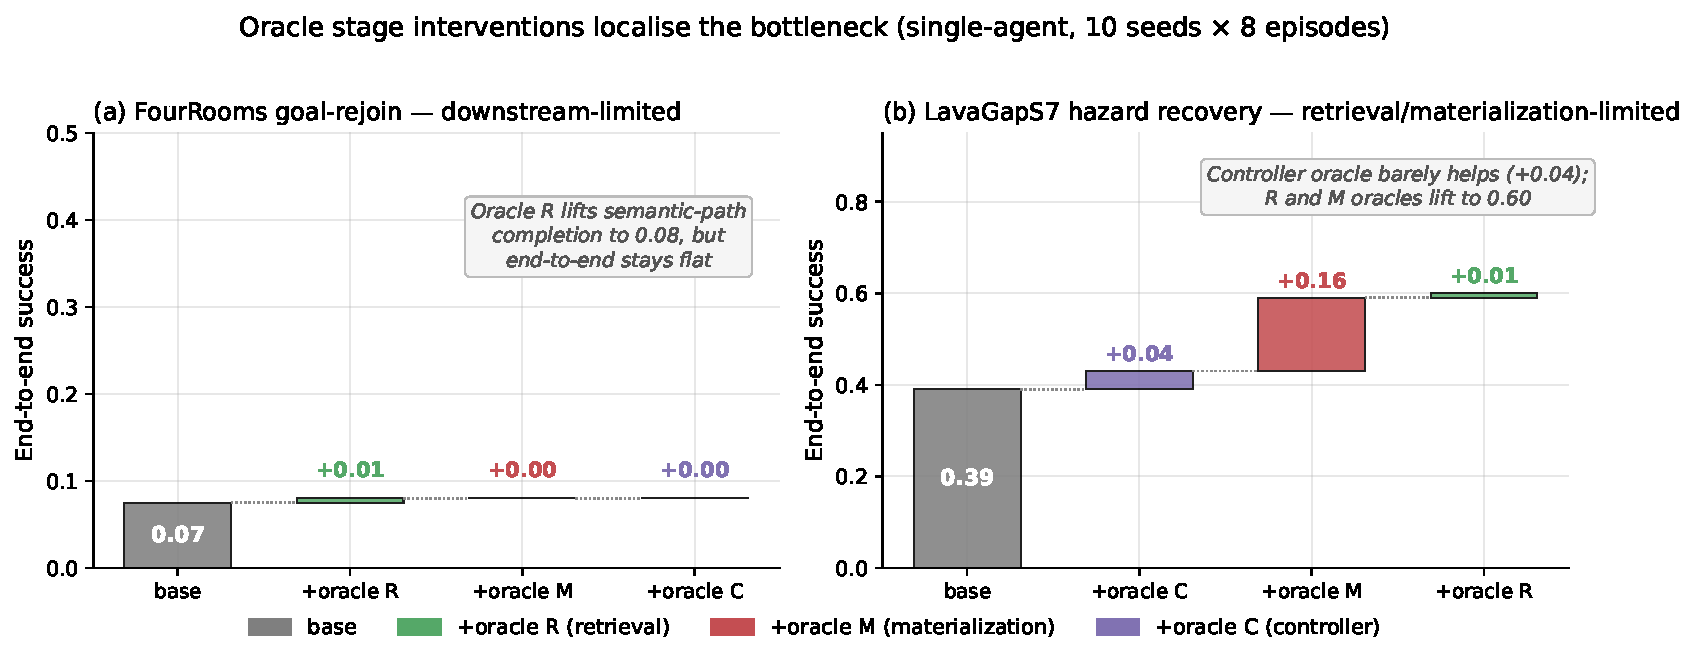
\includegraphics[width=0.98\columnwidth]{figures/fig_oracle_waterfall.pdf}
  \caption{The diagnose$\to$intervene$\to$verify loop on the
  single-agent benchmark: oracle-stage interventions lift exactly the
  stage the decomposition indicts. Hazard recovery is
  retrieval-limited (oracle-R: $0.39\!\to\!0.60$ end-to-end);
  goal-region rejoin is downstream-limited (oracle-R rescues
  semantic-path completion, end-to-end unchanged).}
  \label{fig:oracle}
\end{figure}

A learned behaviour-cloning baseline makes the observability point:
competitive success with collapsed stage structure (no explicit
query/lock interface), so end-to-end optimisation trades away exactly
the events the protocol audits.

\section{Multi-Agent: Memory as a Shared Resource}
\label{sec:multi}

\begin{figure*}[t]
  \centering
  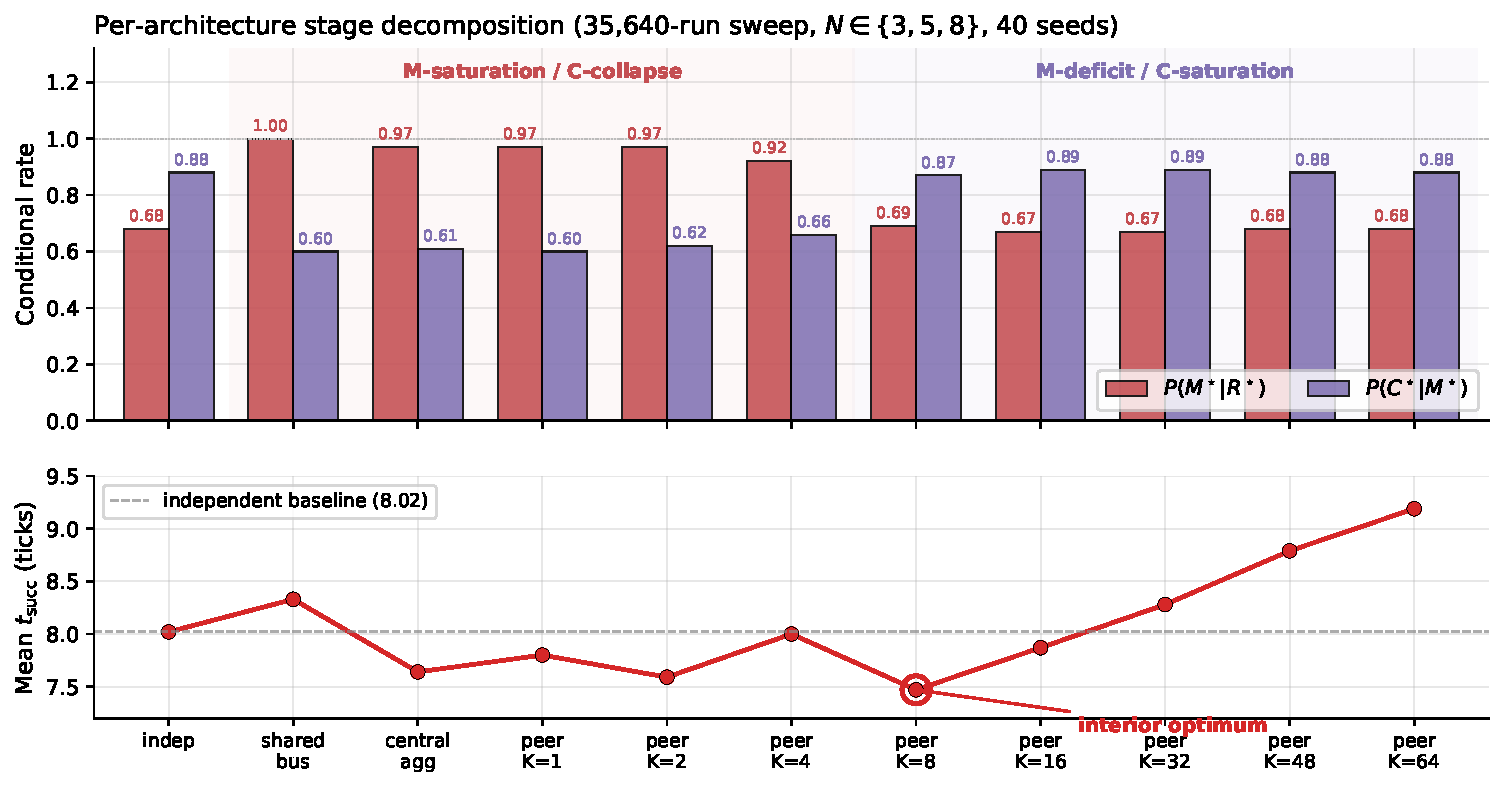
\includegraphics[width=0.92\textwidth]{figures/fig_conditional_rates.pdf}
  \caption{Per-architecture conditional Q/R/M/C rates (top) and mean
  time-to-success (bottom) on the 35{,}640-run sweep. Shared bus,
  central aggregator, and fast peer broadcast ($K{\le}4$) sit in the
  M-saturation/C-collapse regime; independent and slow peer
  ($K{\ge}16$) in the reverse. Time-to-success has an interior minimum
  at $K{=}8$ (7.47 vs.\ 8.02 independent), robust in location, shallow
  in margin.}
  \label{fig:conditional-rates}
\end{figure*}

Four sharing architectures over one symbolic substrate --- independent
private memories, a shared event bus, a central trust-weighted
aggregator, and peer-to-peer broadcast at cadence
$K{\in}\{1,\dots,64\}$ --- run a scarce water-search task
($N{\in}\{3,5,8\}$ agents, $T{\le}N$ targets, three layouts, three
hazard densities, 40 seeds; 35{,}640 runs).
Figure~\ref{fig:conditional-rates} shows the stage profile of every
architecture; retrieval saturates, and all differentiation lives on
the M and C links, as Empirical Claim~1 predicts.

\textbf{Bottleneck shift.} Across peer runs, Spearman of
$P(M^\star|R^\star)$ vs.\ $K$ is $-0.53$ (cluster-robust 95\% CI
$[-0.59,-0.47]$ over 81 configuration cells) and of
$P(C^\star|M^\star)$ vs.\ $K$ is $+0.43$ ($[+0.37,+0.50]$). The
sharper signature is within-cadence: Pearson between the two links
inside a fixed $K$ peaks at $-0.61$ at $K{=}4$ and decays to noise by
$K{=}64$ --- the bottleneck migrates between stages within the same
configuration as $K$ varies. Scaling to $N{=}12$ \emph{sharpens} the
signature (peak $-0.70$, migrating to $K{=}8$). On mean
time-to-success the trade-off produces an interior optimum at $K{=}8$;
consolidation rate is a real, tunable design axis. Oracle
interventions close the loop: at fast cadence, oracle-R/M/C
progressively remove the excess time, attributing it to the
M$\leftrightarrow$C transition.

\begin{figure}[t]
  \centering
  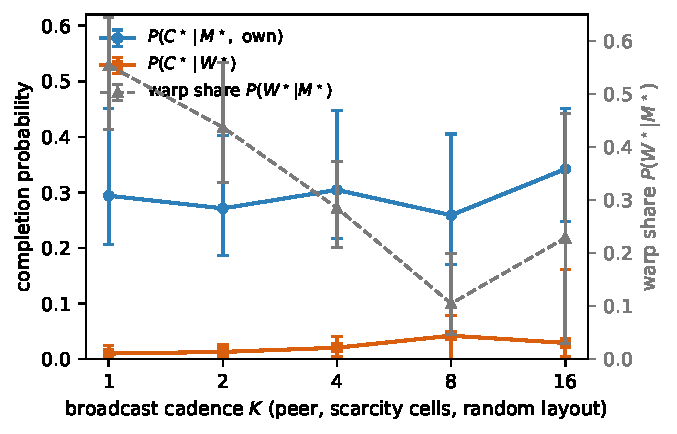
\includegraphics[width=0.98\columnwidth]{figures/fig_warp_strata.pdf}
  \caption{Provenance stratification of $P(C^\star|M^\star)$ vs.\
  cadence $K$ (peer, scarcity cells, episode-cluster bootstrap CIs).
  The share of locks backed by foreign evidence (warp share, grey)
  grows as sharing accelerates, while that stratum's completion
  (orange) stays below $0.05$ and the own-evidence stratum (blue)
  stays flat: the C-collapse of fast sharing is concentrated in the
  foreign-evidence stratum.}
  \label{fig:strata}
\end{figure}

\textbf{The mechanism is provenance.} Annotating each $M^\star$ with
the foreign share $\varphi$ of its supporting evidence mass (computed
from the merge's own weights, frozen at lock time) and calling locks
with $\varphi{\ge}0.8$ \emph{warps}: the warp share falls from $0.55$
at $K{=}1$ to $0.11$ at $K{=}8$ while own-evidence locks complete at a
flat $0.26$--$0.34$ and warp locks below $0.05$ throughout. The
C-collapse of fast sharing concentrates in the foreign-evidence
stratum --- cadence controls how much of the collective's commitment
runs on peers' evidence, and that is the stratum that loses the
occupancy race. The same curve reproduces on a continuous VMAS bridge
($0.72\!\to\!0.00$) and on an LLM text substrate ($0.42\!\to\!0.08$).

\textbf{Learned and LLM collectives.} A CommNet-PPO baseline matches
symbolic peer success ($0.667$ vs.\ $0.65$) with structurally
degenerate stages (its real-valued channel is never informatively
empty; R/M collapse) --- competitive success, zero stage
observability. A collective of three LLM agents (llama3.1) sharing
symbolic memory reproduces the phenomenology on language: pairing
against a no-communication baseline on identical layouts, raw sharing
\emph{lowers} success $2/3\!\to\!1/3$ (occupancy racing), and a
decentralized reservation-and-rollback protocol recovers part of it
($0.33\!\to\!0.42$) with rollback latency ${\approx}K$. On a
step-budget sweep with two local models, an opaque success collapse
($1.00\!\to\!0.00$) resolves to pure C-stage failure
($Q^\star{=}R^\star{=}M^\star{=}1$, $C^\star{=}0$) identically for
both models: a structural, not model-specific, diagnosis.

\section{The Contract on Third-Party Agent Stacks}
\label{sec:external}

\begin{figure*}[t]
  \centering
  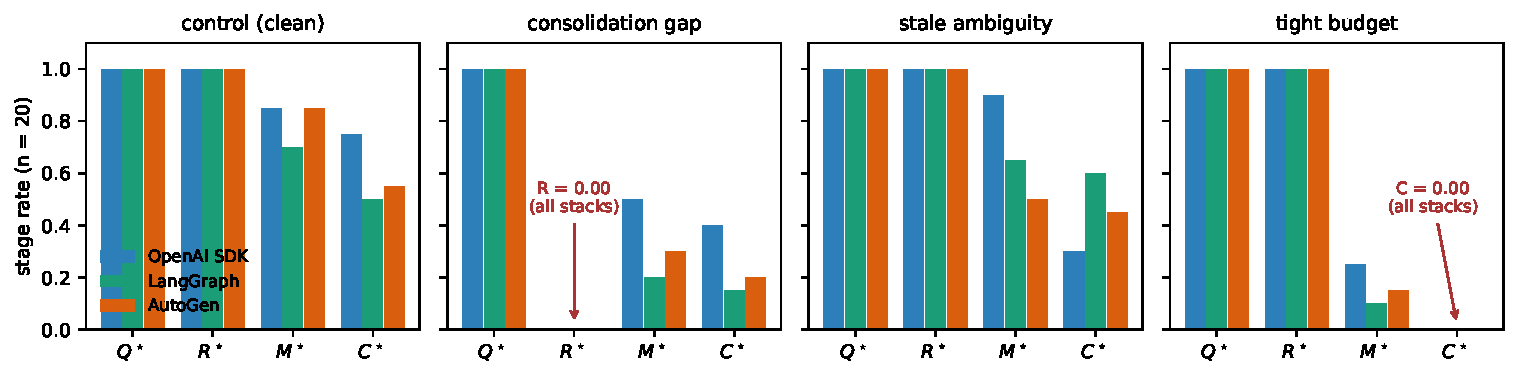
\includegraphics[width=0.92\textwidth]{figures/fig_external_stages.pdf}
  \caption{Stage profiles of three third-party stacks on four
  engineered variants (llama3.1, $n{=}20$/cell). Q and R saturate
  identically; the structural failures give exact zero columns on
  every stack; the inter-framework spread lives in M and C.}
  \label{fig:external-stages}
\end{figure*}

Does the protocol work on systems we did not build? We instrument
three stacks --- an OpenAI-SDK function-calling loop, LangGraph's
ReAct agent, and AutoGen --- with the identical contract defined once
over \emph{tool traces}: an episodic household memory behind
\method{recall}/\method{goto}/\method{take} tools; $Q^\star$ on
querying, $R^\star$ on attribution (a returned record names the item
at its true place), $M^\star$ on an episode-level lock, $C^\star$ on
completion within a tool budget. Four variants engineer one failure
each; all predictions were registered before the runs, and two
revisions of the event semantics are recorded in the registration.

\begin{table}[t]
\caption{Q/R/M/C on third-party stacks (20 episodes/cell). $M_1$:
first commitment targets the true place.}
\label{tab:external}
\centering
\small
\setlength{\tabcolsep}{3.4pt}
\begin{tabular}{llccccc}
\toprule
Stack & Variant & $Q^\star$ & $R^\star$ & $M^\star$ & $C^\star$ & $M_1$ \\
\midrule
OpenAI & control      & 1.00 & 1.00 & .85 & .75 & .25 \\
SDK    & consol.\ gap & 1.00 & \textbf{.00} & .50 & .40 & .25 \\
       & stale ambig. & 1.00 & 1.00 & .90 & .30 & .25 \\
       & tight budget & 1.00 & 1.00 & .25 & \textbf{.00} & .25 \\
\midrule
Lang-  & control      & 1.00 & 1.00 & .70 & .50 & .50 \\
Graph  & consol.\ gap & 1.00 & \textbf{.00} & .20 & .15 & .10 \\
       & stale ambig. & 1.00 & 1.00 & .65 & .60 & .50 \\
       & tight budget & 1.00 & 1.00 & .10 & \textbf{.00} & .10 \\
\midrule
Auto-  & control      & 1.00 & 1.00 & .85 & .55 & .45 \\
Gen    & consol.\ gap & 1.00 & \textbf{.00} & .30 & .20 & .15 \\
       & stale ambig. & 1.00 & 1.00 & .50 & .45 & .35 \\
       & tight budget & 1.00 & 1.00 & .15 & \textbf{.00} & .15 \\
\bottomrule
\end{tabular}
\end{table}

Three findings (Table~\ref{tab:external},
Fig.~\ref{fig:external-stages}). \textbf{(1)~Structural localizations
are exact and framework-independent}: no consolidated fact
$\Rightarrow R^\star{=}0.00$; budget below requirement
$\Rightarrow C^\star{=}0.00$ at $Q^\star{=}R^\star{=}1$ --- $20/20$
episodes on every stack, no per-framework adaptation.
\textbf{(2)~The clean control separates the stacks, and the stages say
how.} Success on identical clean episodes spreads $0.50$--$0.75$. A
leaderboard reports ``different quality''; the stages show a shared
pathology --- first-commitment discipline is weak everywhere
($M_1{=}0.25$--$0.50$: the first \method{goto} frequently ignores the
agent's own just-retrieved evidence) --- plus different loop
economics: episode-level M recovers to $0.70$--$0.85$ by re-query, and
the stacks differ in how much survives to completion ($C/M$ from
$0.88$ down to $0.65$). \textbf{(3)~The stale distractor pulls,
unevenly.} An outdated record captures the first commitment in
$0.20$--$0.40$ of ambiguous episodes, and its completion cost is
framework-specific (OpenAI SDK: $0.75\!\to\!0.30$; the others absorb
the detour). Registered behavioural predictions that assumed a clean
control failed \emph{because the stacks themselves fail a clean memory
task 25--50\% of the time} --- finding~(2), reported as registered
failures with mechanisms.

\textbf{Model robustness (registered before the runs).} Repeating all
240 episodes with a second model (qwen3:4b) confirms the registered
prediction \emph{exactly}: both structural localizations transfer
unchanged ($R^\star{=}0.00$ under the consolidation gap and
$C^\star{=}0.00$ under the tight budget, $20/20$ on every stack). The
behavioural profile, by contrast, is a MODEL property that the stages
make legible: qwen3:4b completes every clean episode
($C^\star{=}1.00$ on all three stacks) with first-commitment
discipline $M_1{=}0.90$--$0.95$ where llama3.1 managed
$0.25$--$0.50$, and is barely distracted by the stale record
($0.05$--$0.30$) --- \emph{except} under AutoGen, which drops qwen's
$M_1$ to $0.40$: the decomposition separates what the model
contributes from what the framework destroys. Full second-model table
in the supplement.

\section{Related Work}

Cognitive-map and semantic-map lines motivate explicit place
abstraction \citep{tolman1948cognitive,gupta2017cognitive,
savinov2018semi}; goal-conditioned RL conditions on goals or
embeddings \citep{andrychowicz2017hindsight}; multi-agent RL studies
learned channels \citep{sukhbaatar2016commnet,foerster2018ctde} and
gossip protocols \citep{boyd2006gossip}; LLM-agent systems add
explicit memory layers evaluated end-to-end
\citep{wang2023voyager,shinn2023reflexion,packer2023memgpt,
park2023generative,wu2023autogen}. The protocol is orthogonal to all
four lines: it does not propose an architecture; it makes any of them
stage-diagnosable from logs, and yields a slope-level cadence
prediction testable on those logs.

\section{Limitations}

Primary substrates are grid worlds; VMAS is a directional continuous
check; the LLM studies use small local models at modest $n$; place
identity across agents assumes a shared coordinate frame (removed
constructively in a companion manuscript); Empirical Claim~1 remains
slope-level --- a derivation under a generative model would make it a
theorem. Full tables, proofs of the estimability arguments,
assumption stress tests, effect-size methodology, scale-up, and all
registered-prediction files are in the supplement.

\section{Conclusion}

Q/R/M/C turns ``the agent's memory failed'' from a scalar verdict
into a located, comparable, and sometimes repairable diagnosis: a
consolidation limit in a single agent, an occupancy-priced sharing
rate in a collective, a commitment-discipline gap in off-the-shelf
agent stacks. The protocol costs a logging contract, not a new
architecture --- and the same four numbers read across symbolic,
learned, and LLM systems.

\bibliography{aaai27refs}

% Reproducibility checklist (pages beyond the 7-page technical limit
% are permitted for references and the checklist).
\def\isChecklistMainFile{}
\input{ReproducibilityChecklist_qrmc_aaai27.tex}

\end{document}
